\section{Trends in humanoid robotics}

The word ``Robot'' first appeared in Karel Capek's 1921 play \textit{Rossum's Universal Robots} where the \textit{robots} were human-like machines made to replace human workers. It comes from the Czech word ``Robota'' which means ``labour doing compulsory manual works without receiving any remuneration'' or ``to make things manually''. Robots are now very widely used in the manufacturing sector. Robotic technology has been developed and refined so successfully that an entire manufacturing process can be handled by robots alone.

The International standard ISO 3873 defines ``Robot'' as: ``An automatically controlled, reprogrammable, multi-purpose, manipulator, programmable in three or more axes, which may be either fixed in place or mobile for use in industrial automation applications''. This definition restricts the area to only one type of robot, the industrial manipulator. But the inclusion of the perception of the environment and a capacity for action with some level of autonomy the robot leaves the manufacturing plant. The continuous evolution of robots needs a more general definition to include other types of robots in the global robotics area. The Oxford dictionary defines ``Robot'' as ``a machine resembling a human being and able to replicate certain human movements and functions automatically''. Nowadays, the robot is leaving factories and laboratories and slowly entering society in the form of a service robot.

\subsection{General classification of robots}
The development of robotics through the ages, makes necessary to do a classification. Based on their ability to make different types of motion, their control architectures differ radically. Five groups of robotic systems can be distinguished by their motion control architecture: industrial, mobile, zoomorphic, anthropomorphic and hybrid robots.

\textit{Industrial robots}. The main characteristic of this group is that all robots are stationary. Industrial robots, including industrial manipulators (Figure \ref{fig:abb}) , are usually designed taking into account different requirements for velocity, load capacity, accessibility, etc. and always have a limited number of degrees of freedom. These robots are structured to move their end effectors in a determined working environment in one or several systems of coordinates. Although, exceptions may exist when a robot is guided in space (with moving platform) in order to perform a task in another environment. These robots are used when it is necessary to attend rather extensive but permanent working zones, working mainly with different types of objects and environments and does not exist human-robot interaction.
\begin{figure}[!hbt]
\centering
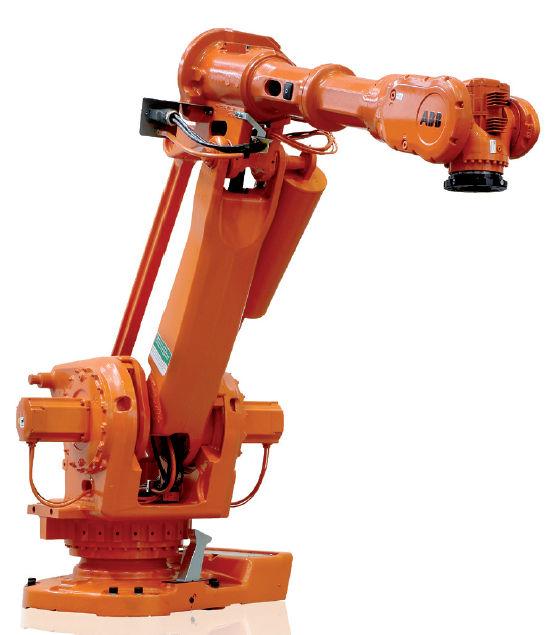
\includegraphics[scale=0.25]{abb.jpg}
\caption{ABB industrial manipulator}
\label{fig:abb}
\end{figure}
 
\textit{Mobile robots}. This group has more motion capacity due to implemented wheel based platform systems (Figure \ref{fig:mobile}). They can execute different telecontrolled tasks or are driven by the environmental information received from the integrated sensorial system. 
%The motorized turtle designed in 1948 by Walter was the first predecessor. 
From the beginning of the sixties mobile robots were designed and implemented within industry. These robots were able to transport parts from one point of the production line to another, guided by preplanned paths materialized by the electromagnetic or photoelectric bands from circuits mounted into the floor. From the beginning of the seventies a lot of work was related to major autonomy of mobile robots, like providing the mobile robot a vision system. Years later, when more complex and precise sensorial systems appeared, the development of control architectures for mobile robots was concentrated on the superficial intelligence and decision making systems \cite{Malfaz2012}. Mobile robots provided with this kind of control system are usually able to plan motions and avoid obstacles. Today, research is also centred on human-mobile robot interaction \cite{Ramey2011}. 

\begin{figure}[!hbt]
\centering
\subfigure[TurtleBot mobile robot]{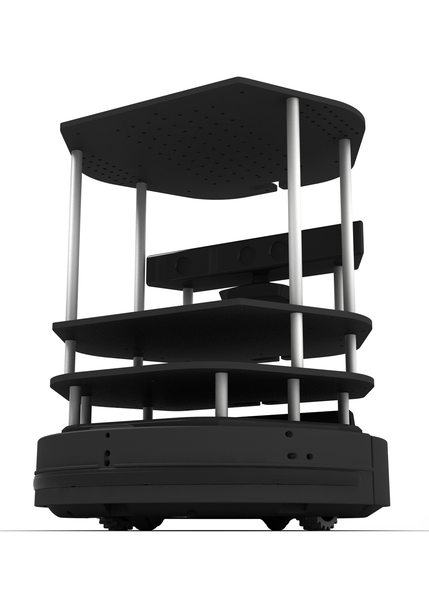
\includegraphics[width=30mm]{turtlebot.png}}\hspace{10mm}
\subfigure[MAGGIE social robot from UC3M]{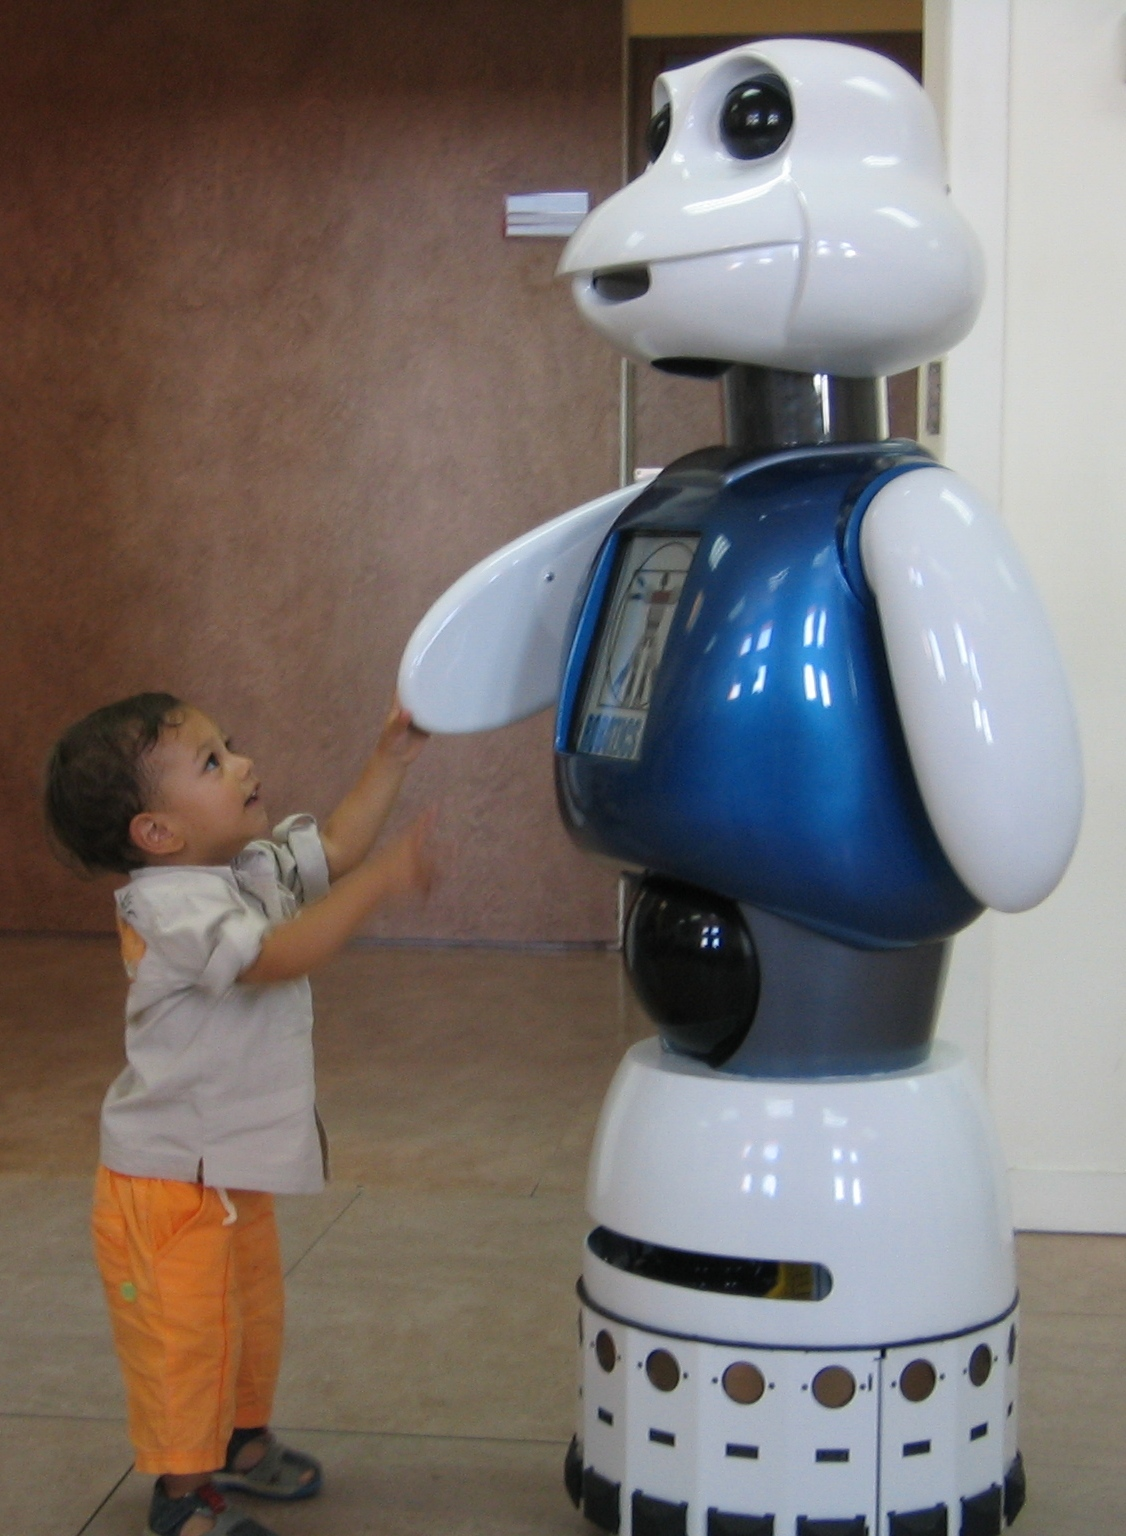
\includegraphics[width=30mm]{maggie.jpg}}
\caption{Mobile robots}
\label{fig:mobile}
\end{figure}

\textit{Zoomorphic robots}. This type of robot is characterized by the locomotion system which imitates the locomotion of diverse living beings. Although there can be a lot of morphological differences between all variations of zoomorphic systems, it is possible to distinguish two basic categories: walking and non-walking zoomorphic architectures. An example of non-walking zoomorphic robot is the modular snake-like robot in Figure \ref{fig:zoo} (a). Walking zoomorphic robots are developed to work in every king of terrain and they have a really wide range of applications.
%It could be spatial research, out-of-the-way terrain exploration, or volcanic research. 
Animal-like robots try to imitate the movements of animals and are usually constructed for research and entertainment. The control of this kind of robot is more complicated than control of a mobile or industrial robot because of the need to maintain the equilibrium at every stage of motion. Figure \ref{fig:zoo} (b) shows the WildCat walking zoomorphic robot developed by Boston Dynamics.

\begin{figure}[!hbt]
\centering 
\subfigure[Non-walking zoomorphic robot]{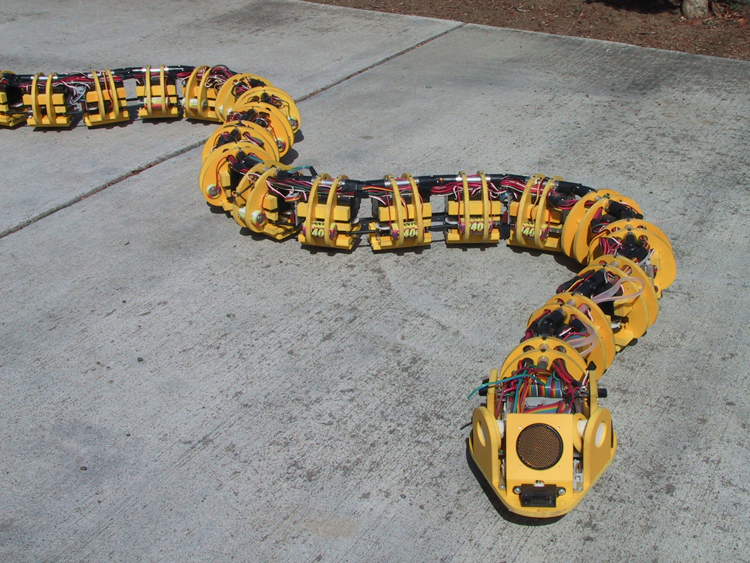
\includegraphics[width=40mm]{snake.jpg}}\hspace{10mm}
\subfigure[WildCat walking zoomporphic robot]{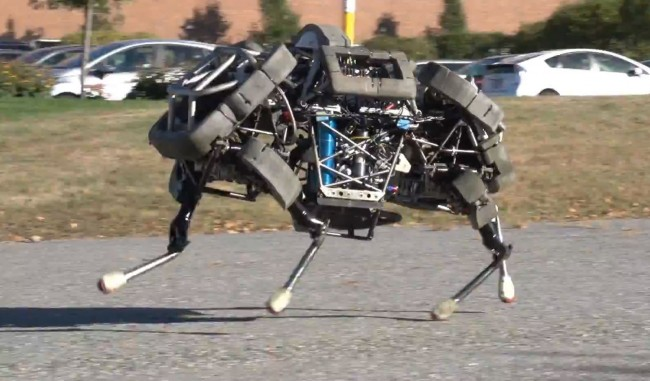
\includegraphics[width=40mm]{wildcat.jpg}}
\caption{Zoomporphic robots}
\label{fig:zoo}
\end{figure}

\textit{Anthropomorphic robots (Androids)} or humanoid (bipedal) robots. These robots try to reproduce the body and behaviour of a human being. Presently the research on humanoids is increasing rapidly, although, there still remains a lot of work ahead. One of the basic challenges in this field is to reproduce human-like motion abilities beginning with the bipedal locomotion. The motion control architecture in this case is the most complex compared with the other robot types presented above. The main challenge is being able to control and coordinate in real time the dynamics of the whole body and maintain the equilibrium in the single support phase, i.e. when the robot is supported only by one foot. The control architecture of this kind of robot is an aim of this research work and will be discussed and developed further in the following chapters. Figure \ref{fig:humanoid} shows two examples of humanoid robots: (a) is Asimo Robot developed by Honda and (b) is TEO robot from UC3M.

\begin{figure}[!hbt]
\centering 
\subfigure[ASIMO robot]{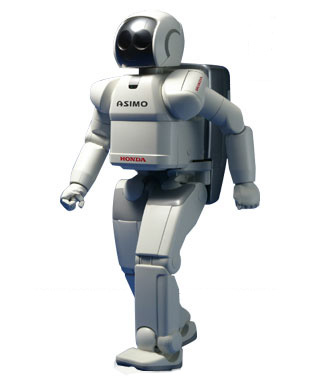
\includegraphics[width=30mm]{asimo.jpg}}\hspace{10mm}
\subfigure[TEO robot]{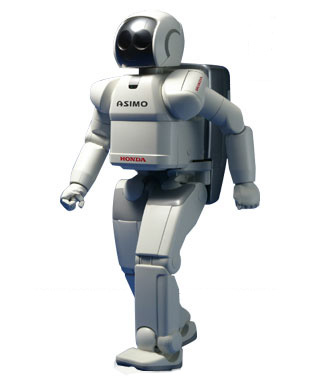
\includegraphics[width=30mm]{asimo.jpg}}
\caption{Humanoid robots}
\label{fig:zoo}
\end{figure}


Another complex aspect related to androids is the ability to reproduce the human upper body, especially the face. The difference between a humanoid robot and android is only skin-deep. The latter looks exactly like a human on the outside, but internally has the mechanics of a humanoid robot. But the human-like appearance can be controversial. In 1970, Masahiro Mori \cite{Mori2012} presented his hypothesis about the \textit{Uncanny Valley} (Figure \ref{fig:valley}). Mori's insight was that people would react with revulsion to human-like robots, whose appearance resembled, but did not quite replicate, that of a real human. The Uncanny Valley has become more relevant in the past few years since robots that actually look and move like humans are starting to become a reality. In fact, researchers currently debate over whether they should try to overcome the uncanny valley or simply design robots that are more mechanical in appearance.

\begin{figure}[!hbt]
\centering
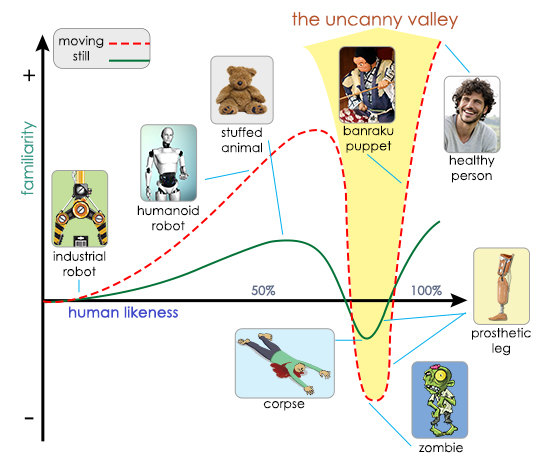
\includegraphics[scale=0.45]{valley.jpg}
\caption{Uncanny valley}
\label{fig:valley}
\end{figure}


\textit{Hybrid robots.} These type  of robots combine properties of various types of other robots. Usually they are a combination of a wheelbase (mobile robot) with an anthropomorphic body. Some examples are Justin robot from the German Aerospace Center (DLR) and TIAGO robot from PAL Robotics (Figure \ref{fig:hybrid}). They are both mainly involved in manipulation tasks (grasping, picking and placing, etc.) and the problem of locomotion in not considered as in humanoids. 

\begin{figure}[!hbt]
\centering 
\subfigure[Justin robot]{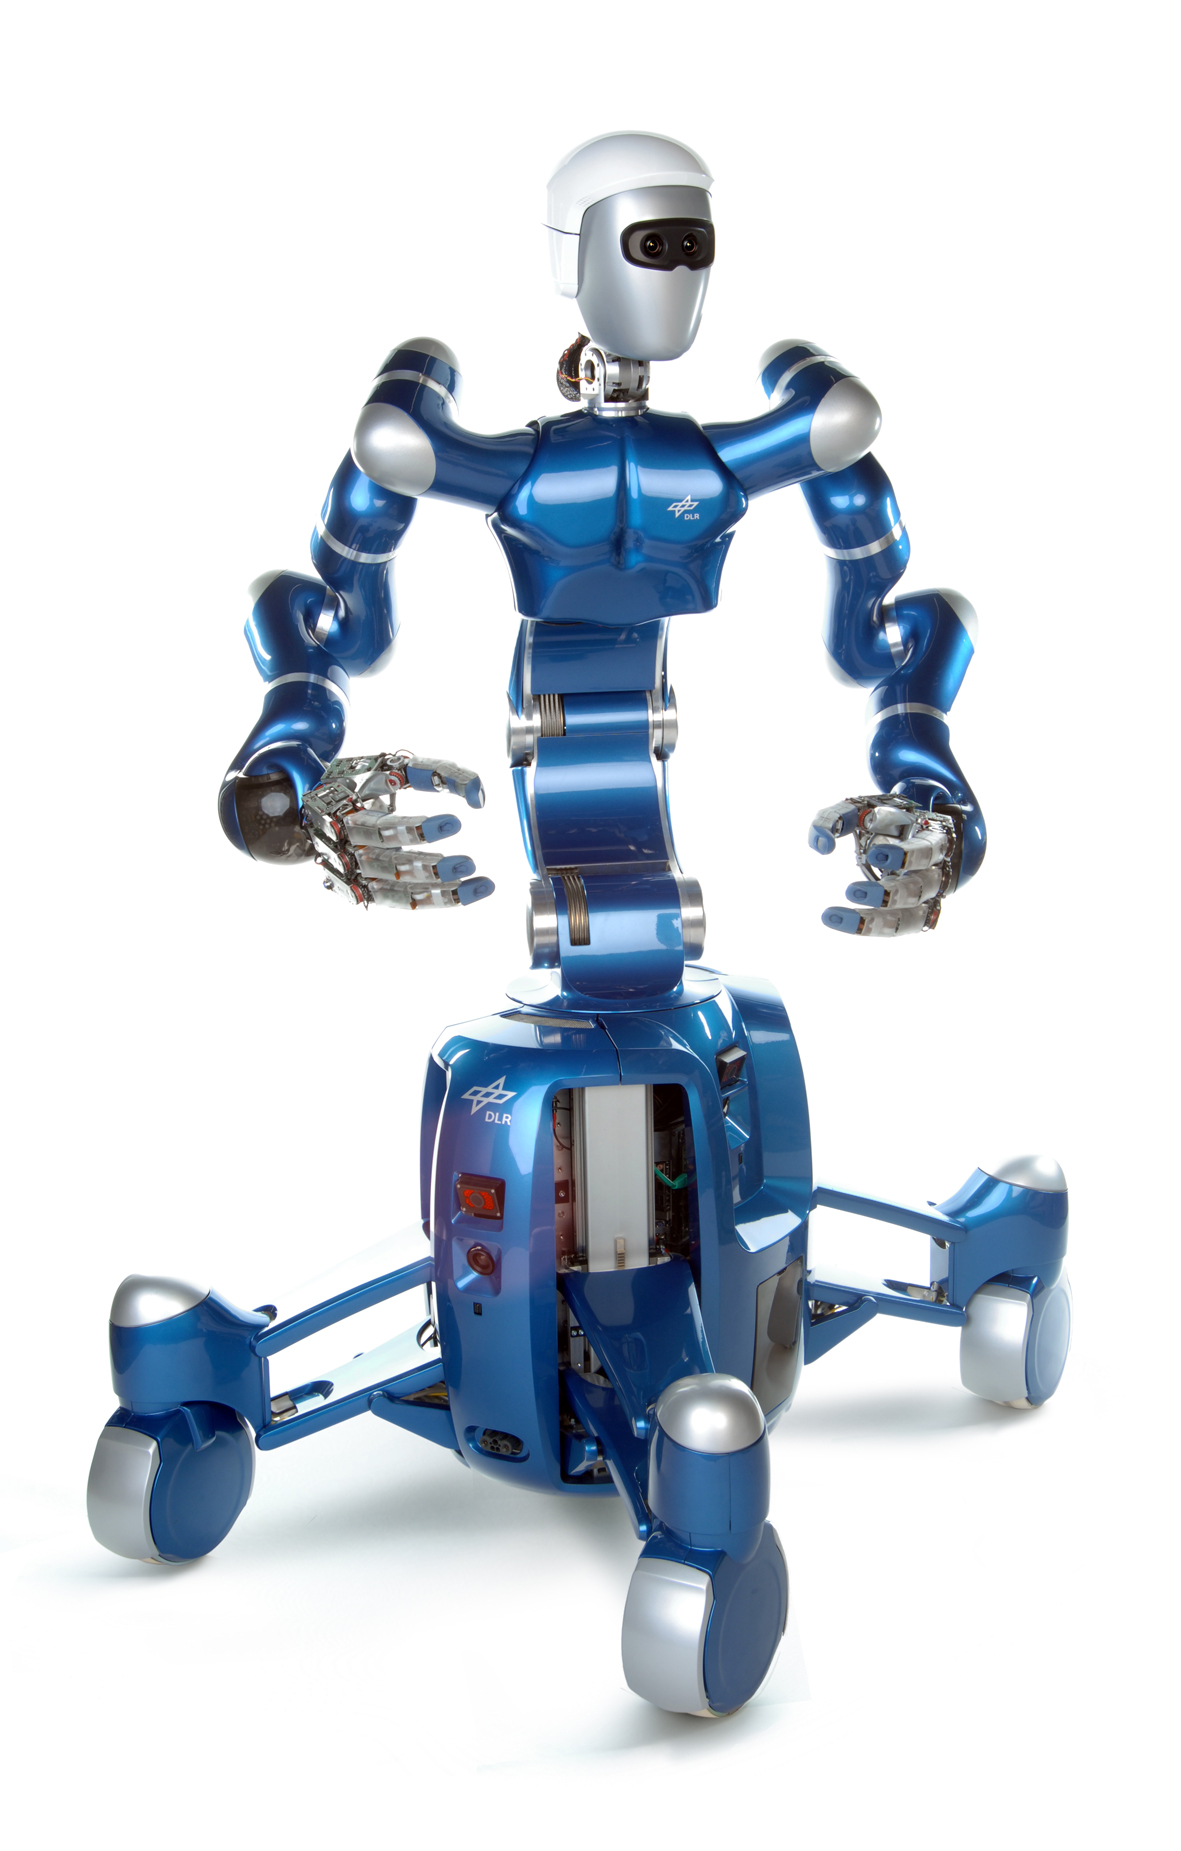
\includegraphics[width=30mm]{justin.jpg}}\hspace{10mm}
\subfigure[TIAGO robot]{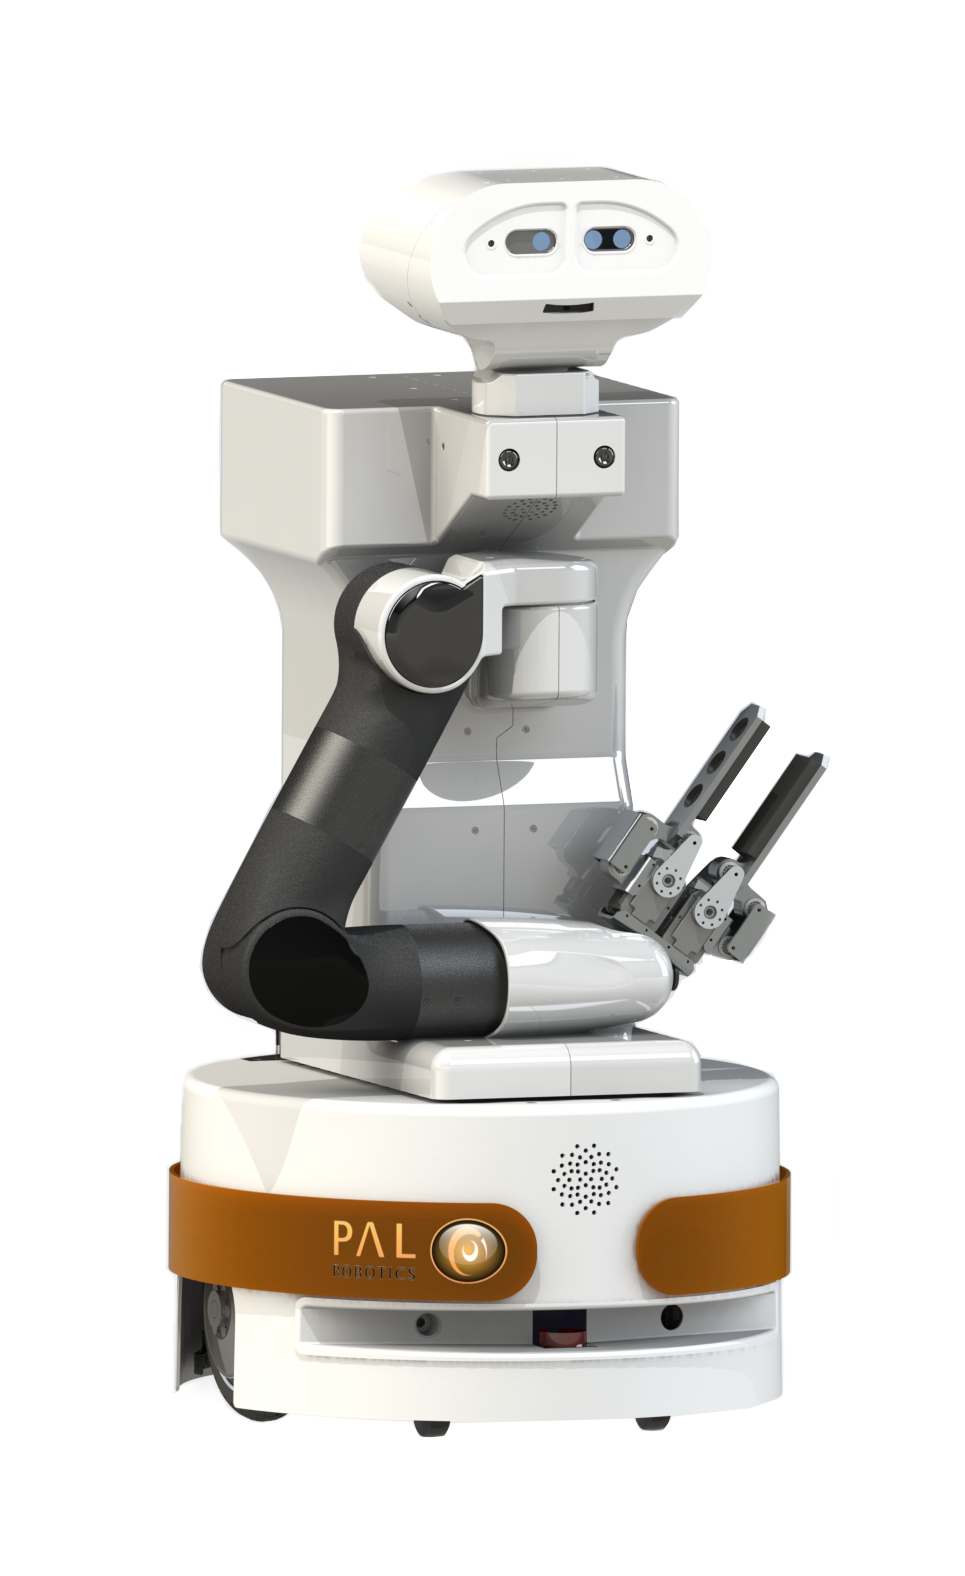
\includegraphics[width=30mm]{tiago.jpg}}
\caption{Hybrid robots}
\label{fig:hybrid}
\end{figure}

\newpage



\subsection{Humanoid robots}

The history of the development of humanoid robots is curiously long and detailed. Leonardo da Vinci designed and possibly built the first humanoid robot (Figure \ref{fig:knight}). The robot, completely mechanical, was designed to sit up, wave arms and move its head via a flexible neck while opening and closing its jaw. 

\begin{figure}[!hbt]
\centering
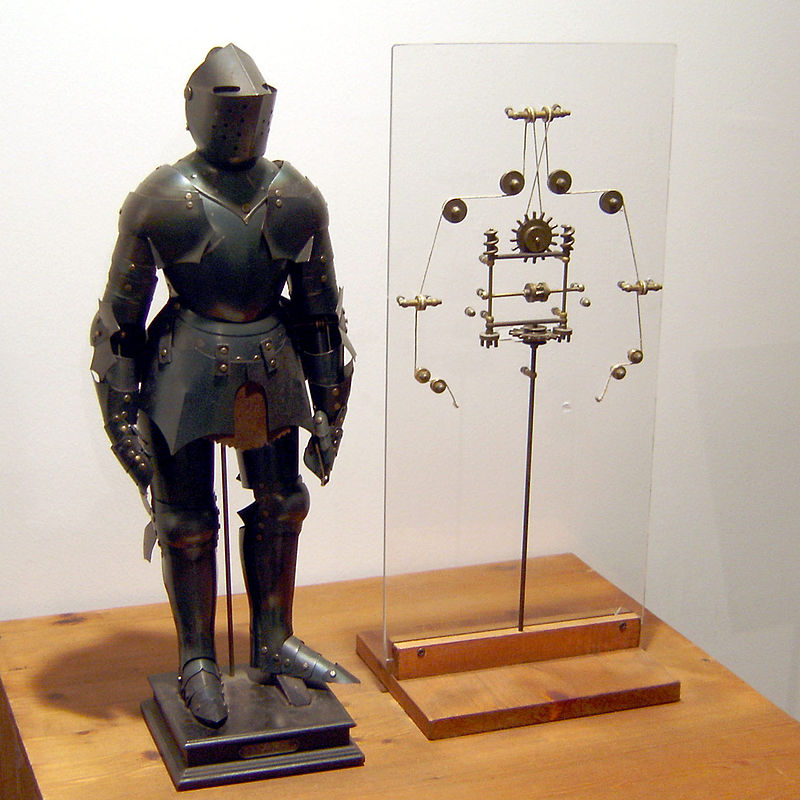
\includegraphics[scale=0.15]{knight.jpg}
\caption{Leonardo da Vinci's mechanical knight}
\label{fig:knight}
\end{figure}

Other designs, related to the appearance of steam power and electricity appeared in the 19\up{th} Century. They were simple automates that imitated some human movements. The first bipedal machine was constructed by George Moore in 1983 but the real progress was achieved only at the end of the 1960s when the electronics, mechanics and materials became sufficiently advance to create such a complex system as a bipedal robot.

In the middle of the 1960s, the Japan University of Waseda launched different research projects lead by Kato and as a result, the series of WL robots appeared. They were only lower body robots (Figure \ref{fig:wl}).

\begin{figure}[!hbt]
\centering 
\subfigure[]{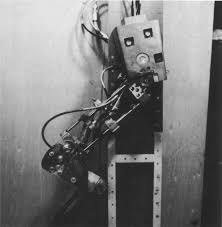
\includegraphics[width=40mm]{wl1.jpeg}}\hspace{10mm}
\subfigure[]{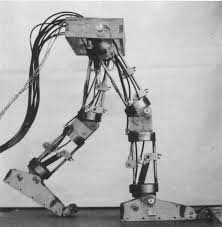
\includegraphics[width=40mm]{wl3.jpeg}}
\caption{(a) WL-1 (b)WL-3}
\label{fig:wl}
\end{figure}

But the real first works about bipedal robots with humanoid appearance (complete torso) were carried out about 1970 by authors Kato \cite{Kaj2005} and Vukobratović \cite{Vuk1970}. The first anthropomorphic robot WABOT-1 (Figure \ref{fig:wabot} (a)), was exhibited by Kato in 1973. Using a very simple control diagram, the robot was able to perform a few slow gaits, maintaining its balance at all times. This achievement, was the first one that encouraged researchers about humanoid robots and their locomotion.

At the same time, Vukobratović and his research team were studying stability in biped systems in the former Yugoslavia, basing on a new stability criterion, presented in 1972, as \textit{Zero-Moment Point (ZMP)} \cite{Vuk2004}. Taking into account the dynamic effects produced during a walking, from then until now, the ZMP stability criterion has been the most used in humanoid or biped robotics.

The second prototype WABOT-2 of Waseda University was developed between 1980 and 1984. The robot musician WABOT-2 can converse with a person, read a normal musical score with its eyes and play tunes on an electronic piano. The WABOT-2 can be mentioned as one of the first personal robots.

\begin{figure}[!hbt]
\centering 
\subfigure[]{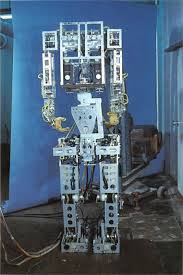
\includegraphics[width=40mm,height=50mm,keepaspectratio]{wabot1.jpeg}}\hspace{10mm}
\subfigure[]{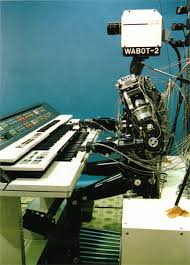
\includegraphics[width=40mm,height=50mm,keepaspectratio]{wabot2.jpeg}}
\caption{(a) WABOT-1 (b)WABOT-2}
\label{fig:wabot}
\end{figure}

Years later, the proyect continued in the Japanese university and the WABIAN series (Figure \ref{fig:wabian}) were constructed as improvements of the previous ones. These robots had advances in their degrees of freedom, better mechanical structure, better stability and bigger weight of objects to be transported. The WABIAN series is still in development with its latest prototype WABIAN 2-R. New technologies and materials make a huge difference between this and the first versions. An important advantage of its mechanical design is the use of 2-DOF in the waist which enables more fluent walking motions. 

\begin{figure}[!hbt]
\centering 
\subfigure[]{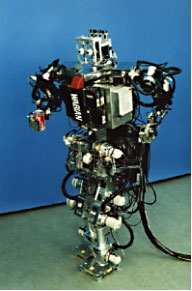
\includegraphics[width=30mm,height=40mm,keepaspectratio]{wabian.JPG}}\hspace{10mm}
\subfigure[]{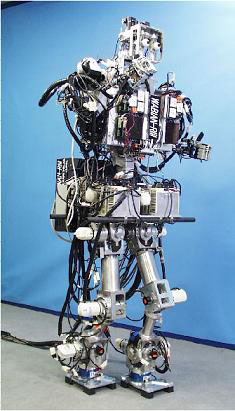
\includegraphics[width=30mm,height=40mm,keepaspectratio]{wabianrv.JPG}}
\hspace{10mm}
\subfigure[]{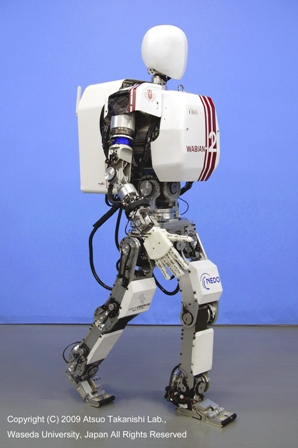
\includegraphics[width=30mm,height=40mm,keepaspectratio]{wabian2r.jpg}}
\caption{(a) WABIAN (b) WABIAN-RV (c) WABIAN-2R }
\label{fig:wabian}
\end{figure}

The development of humanoid robotics was not only at universities also in industry. The Honda Motor Company was one of the main pathfinder industries involved in robotics. In the mid 1980s, they began creating biped walking robots (only lower body parts). But the rise of humanoid robots started with the development of P1 robot in 1993 \cite{Kaj2005}. The project began in secret years before, after the exhibition of WABOT-2 playing the piano. The next version, P2 in 1996 (180 centimetres high and 210 kg weight), was the first humanoid able to walk in a stable enough way and carry its processor and battery on its back. After that, robots P3 and ASIMO were its advanced versions, reducing hight and weight of the robot.


\begin{figure}[!hbt]
\centering
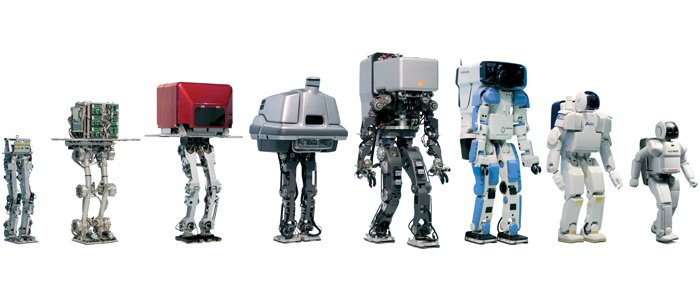
\includegraphics[scale=0.5]{honda.jpg}
\caption{Honda humanoid prototypes. From left to right: E0 (1986) , E1(1987), E3(1989), E5(1992), P1(1993), P2(1996), P3(1997), ASIMO(2000)}
\label{fig:honda}
\end{figure}

Undoubtedly, ASIMO is the culmination of two decades of research in humnaoid robotics by Honda. ASIMO (130 centimetres and 54 kg) is able to run, walk (at 2.7 km/h) on uneven and slope surfaces, climb stairs, grasp objects among other tasks. It also can avoid moving obstacles as it moves through its environment. 

Other of the most advanced humanoid robots is the HRP-2 . The Humanoid Robotics Project (HRP) is led by the National Institute of Advanced Industrial Science and Technology (AIST) and Kawada Industries in Japan \cite{Kaneko2004}. The main outcome of this project was HRP-2 which is taller (140 cm) buth lighter (58 kg) than Honda's Asimo. HRP-2 was the first finished prototype in the HRP series to demonstrate walking (2 km/h maximum speed) on uneven surfaces, getting up from a fallen position and to interact with humans and help in domestic service tasks. Subsequently, HRP-3 was developed based on the HRP-2 experience with additional dust and splash-proof protection, enhanced hand coordination, improved cooling systems, and prolonged operation time. In particular, the prototype of HRP-3 \cite{Kanehiro2006} was developed using a distributed control system and a real-time Ethernet communication network. Later, HRP-4 has a new slim, lighter and athletic mechanical design (weight of 39 kg, height of 151 cm) to improve its functioning in the domestic environment. In addition to the mechanical upgrades, this robot has several key improvements which include LAN and Wireless LAN networks for internal and external communications. Finally, HRP-4c \cite{Kan2011}, also referred to as the cybernetic humanoid robot, is the most recently developed humanoid robot in the HRP series with a female appearance which is 158 cm tall and weighs 43 kg. HRP-4c has human like facial expressions. It should be noted that all the HRP series robots have rigid joints which are controlled by local PID controllers and an online ZMP based trajectory generation.

\begin{figure}[!hbt]
\centering 
\subfigure[HRP-2]{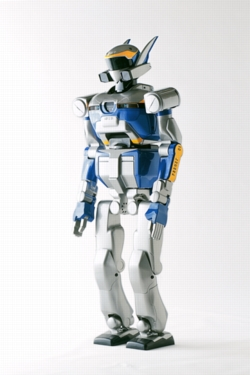
\includegraphics[width=30mm,height=40mm,keepaspectratio]{HRP2.jpg}}\hspace{5mm}
\subfigure[HRP-3]{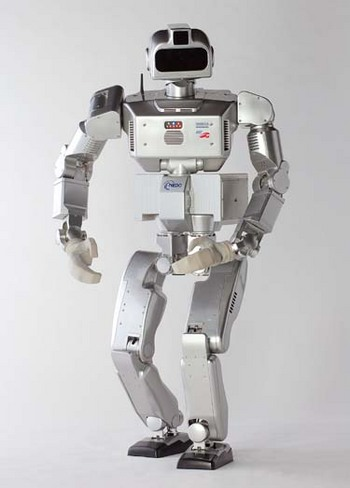
\includegraphics[width=30mm,height=40mm,keepaspectratio]{HRP3.JPG}}
\hspace{5mm}
\subfigure[HRP-4]{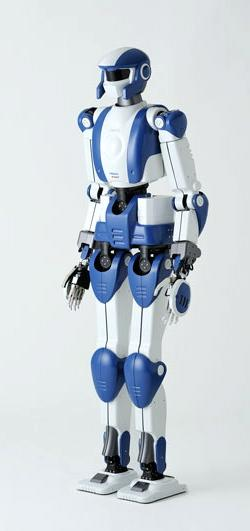
\includegraphics[width=30mm,height=40mm,keepaspectratio]{HRP4.jpg}}
\hspace{5mm}
\subfigure[HRP-4c]{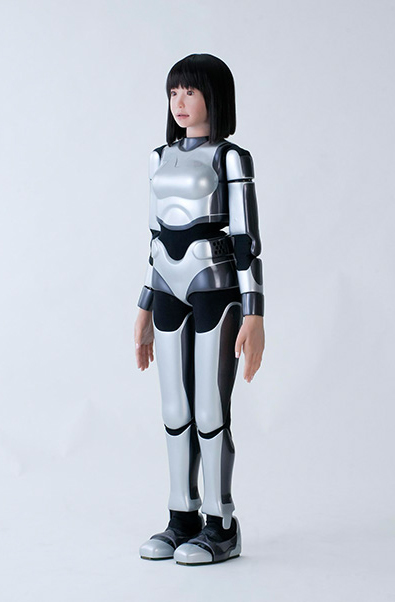
\includegraphics[width=30mm,height=40mm,keepaspectratio]{HRP4c.jpg}}
\caption{HRP series}
\label{fig:hrp}
\end{figure}

Meanwhile, the Korean Advanced Institute of Science and Technology (KAIST) has been developing a series of walking robots since 2001 which consist of KHR-1, KHR-2 and KHR-3 where the mechatronic design was evolved over three versions. Hubo (KHR- 3) is the latest humanoid robot developed at KAIST in 2004 which has 41 DoF, stands 125 cm tall and weighs 55 kg as shown in Figure \ref{fig:hubo} (a). The aim of the Hubo project is to provide a reliable platform for implementing dynamic walking, navigation and image processing algorithms \cite{Park2007}. In 2008, Hubo was integrated with an android head resembling Albert Einstein. The head used RC servo motors for facial expressions and the robot was called Albert Hubo \cite{Park2008} (Figure \ref{fig:hubo} (b)). In late 2009, a running experiment was reported on Hubo \cite{Cho2009} with the maximum speed of 3.24 km/h. The tracking control system which used in Hubo humanoid robot is based on independent PD position feedback loops running at 1 kHz which is the traditional approach for trajectory tracking in robotics.

\begin{figure}[!hbt]
\centering 
\subfigure[]{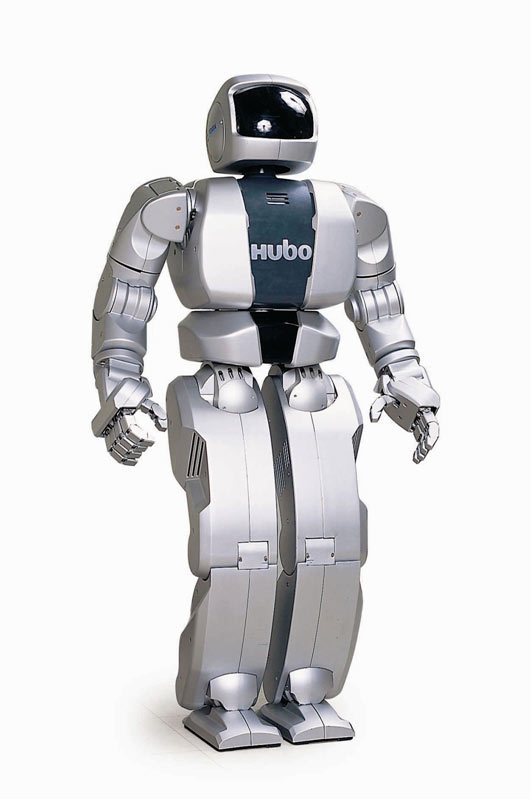
\includegraphics[width=40mm,height=50mm,keepaspectratio]{hubo.jpg}}\hspace{10mm}
\subfigure[]{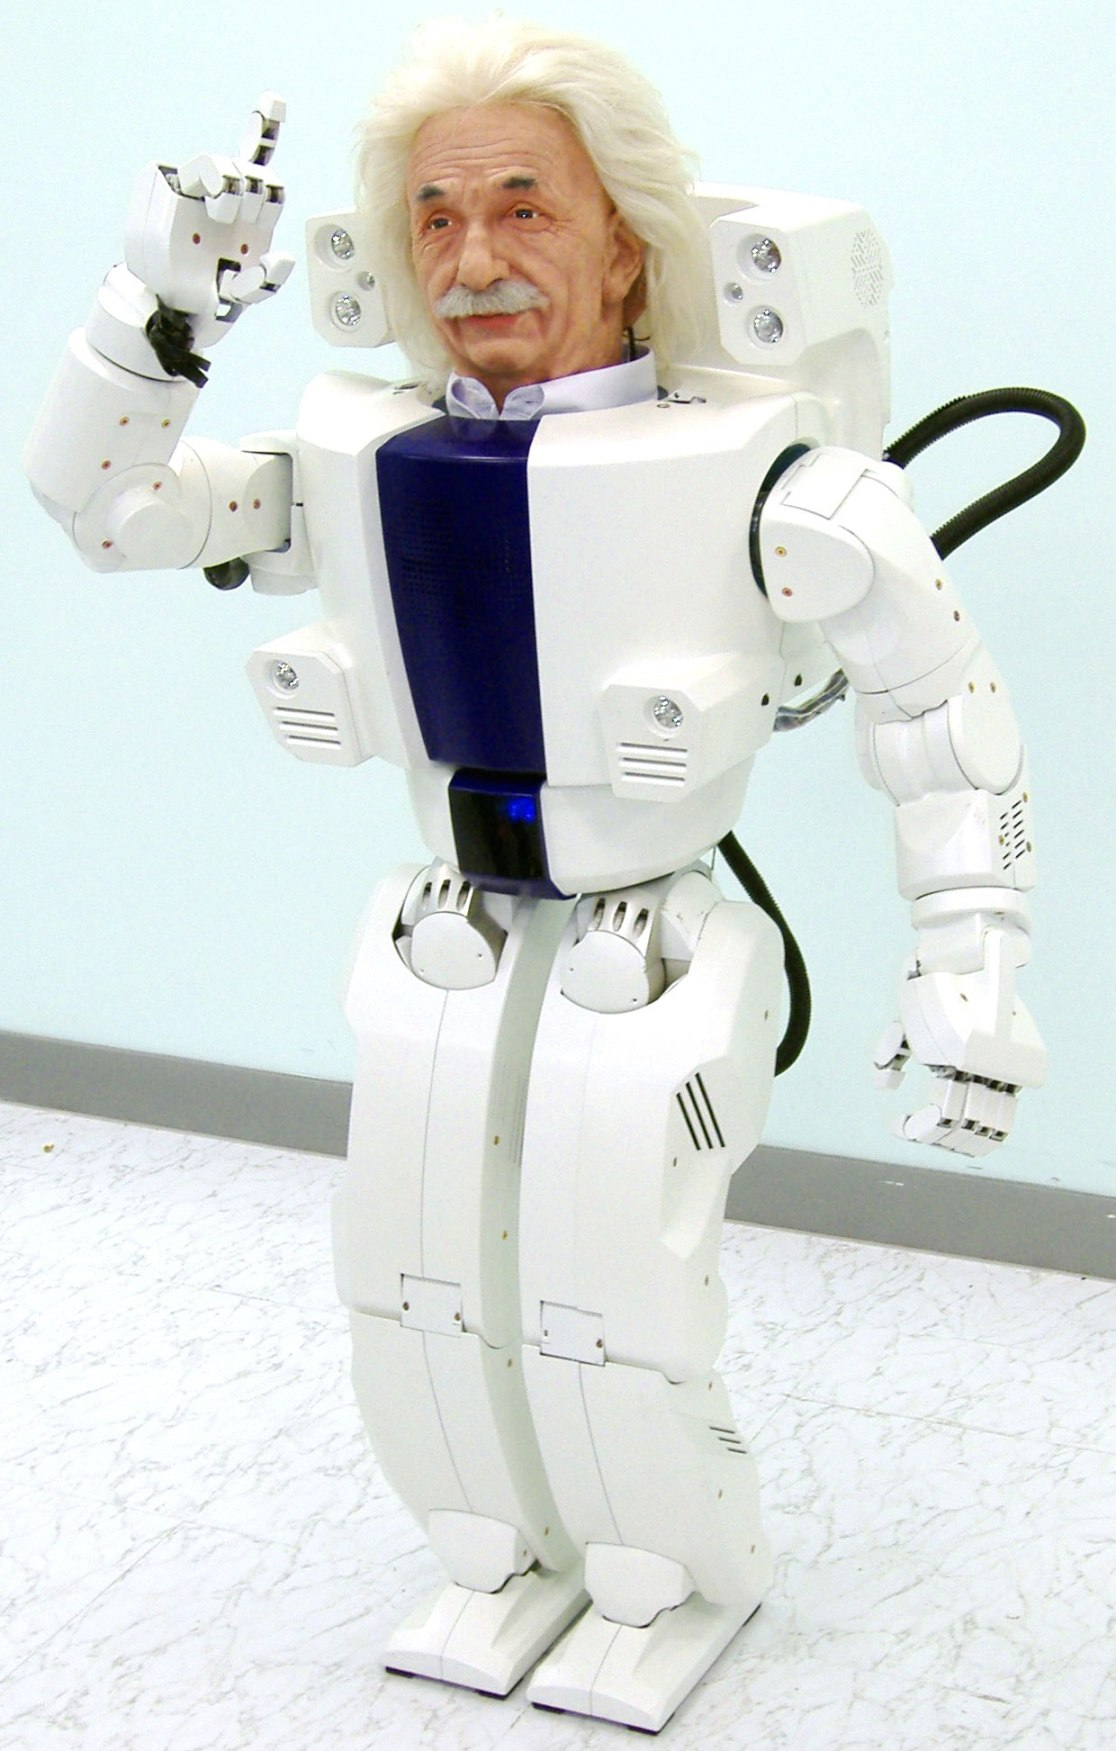
\includegraphics[width=40mm,height=50mm,keepaspectratio]{AlbertHubo.jpg}}
\caption{(a) HUBO robot (b)Albert HUBO robot}
\label{fig:hubo}
\end{figure}


The fastest walking robot is Petman by Boston Dynamics with a human like walking speed of 4.4 miles per hour (7 km/h approx.) \cite{BostonWeb}. The aim of the Petman project is to study the feasibility of chemical testing using a fully articulated robotic mannequin for the US military. Petman weighs 80 kg and stands about 1.75 m tall and has hydraulic actuators which in addition to high power output, provide a degree of compliance to absorb the ground impacts. Currently the robot can walk, go up the stairs, squat and kneel. Recently, Boston Dynamics has received more funding from DARPA (Defense Advanced Research Projects Agency in USA) to develop a more advanced version of Petman which is called Atlas.

\begin{figure}[!hbt]
\centering 
\subfigure[]{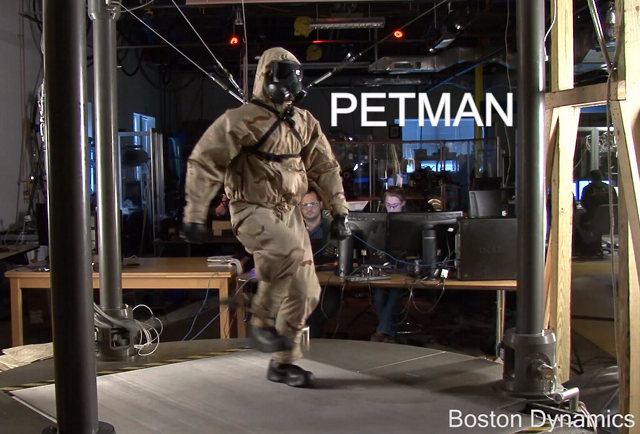
\includegraphics[width=80mm,height=50mm,keepaspectratio]{petman.jpg}}\hspace{10mm}
\subfigure[]{\includegraphics[width=40mm,height=50mm,keepaspectratio]{atlas.jpg}}
\caption{(a) PETMAN robot (b)ATLAS robot}
\label{fig:boston}
\end{figure}


Going to small sized humanoid robots, iCub (from the Instituto Italiano di Tecnologia) is a humanoid robot that was developed in five years by the RobotCub \cite{icubWeb} consortium to provide the cognitive science research community with an open source platform to study cognition. In other words, iCub is used as an open source robotic platform to study how a human child learns the basic motor skills as well as learning and recognizing different objects. iCub is a full humanoid robot with a head, arms, hands, waist, and legs that are actuated by 53 motors. It is the size of a 3.5 year old child with a compact, modular, mechatronic architecture, stands 104 cm tall, and weighs less than 23 kg. Its internal communication network is based on CAN, which connects the local DSP joint controllers to the central computer located at its head.

Other open-source small sized humanoids (Figure \ref{fig:mini}) are NAO humanoid robot (58 cm, 4.3 kg and 21 to 15 DoF) developed by Aldebaran Robotics in Paris, the Fujitsu  HOAP-3 humanoid robot (60 cm and 8.8 kg), and the DARwIn-OP (54.5 cm, 2.9 kg, 11 DoF) developed by RoMeLa at Virginia Tech in collaboration with the University of Pennsylvania, Purdue University and Robotis Co.

\begin{figure}[!hbt]
\centering 
\subfigure[iCub]{\includegraphics[width=60mm,height=40mm,keepaspectratio]{icub.JPG}}
\hspace{5mm}
\subfigure[NAO]{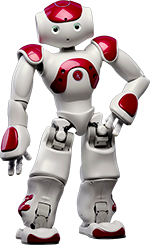
\includegraphics[width=30mm,height=40mm,keepaspectratio]{nao.png}}
\hspace{5mm}
\subfigure[DARwIn]{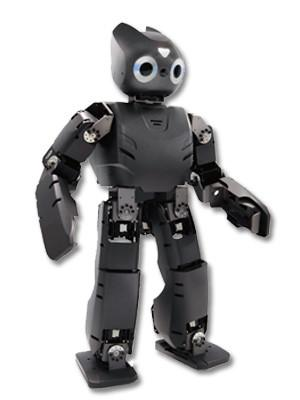
\includegraphics[width=30mm,height=40mm,keepaspectratio]{darwin.jpg}}
\hspace{5mm}
\label{fig:mini}
\caption{Mini humanoids robots}
\end{figure}

In Spain, two main projects are being developed. On the one hand the company PAL Robotics develops humanoid robot REEM-C \ref{fig:pal} which is 1.65 m tall  and wheighs 80 kg. This robot has grasping ability, object and faces recognition, obstacle avoidance, human-robot interaction and speech and voice recognition in several languages. It is fully compatible with ROS (Robotic Operating System).

\begin{figure}[!hbt]
\centering
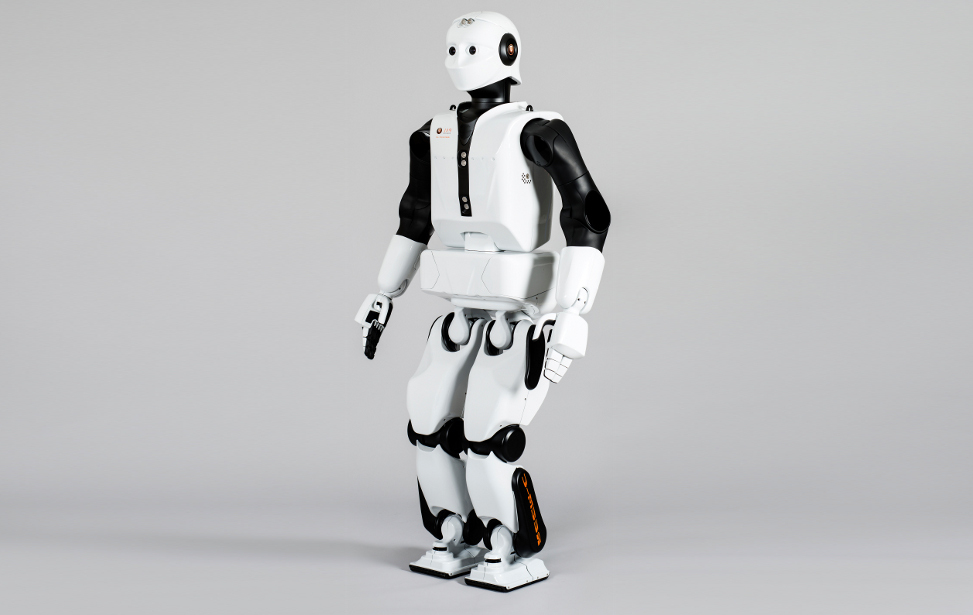
\includegraphics[scale=0.2]{pal.jpg}
\caption{REEM-C robot from PAL Robotics}
\label{fig:pal}
\end{figure}

On the other hand, the Robotics Lab of the University Carlos III of Madrid launched the humanoid robot project, the Rh-0 in its first phase (2002-2004), the Rh-1 (2005-2007) and finally the Rh-2 (2007-Present). The Rh-1 humanoid robot \ref{fig:rh} is 1.45 m tall, weighs 48.5 kg, has 21 DOFs, can walk at about 0.8 Km/h \cite{Arbulu2005}, recognizes faces, and responds to voice commands. The Rh-2 is an improvement of its previous version and it is 165 cm tall, wheighs about 63 kg and it has 26 DoF. This platform is the one used in the experimental trials of this work, so its technical characteristics will be seen in Section \ref{cap:platform_description}.

%The Control level is divided into 3 layers represented as a controller centered on its own task, such as external communications, motion controller’s network supervision, or general control. At on the Device level, each servo drive not only closes the servo loop, but also calculates and performs trajectories online, synchronizes with other devices, and can execute different motion programs located in its memory. These kinds of devices are located near the motors, gaining the benefit of less wiring that is one of the requirements for energy efficiency. They are light-weight and require less effort in cabling. Advanced and commercially available motion controllers were utilized in order to reduce development time and cost. Continuous evolution and improvements in electronics and computing have already made it possible to reduce the industrial controller’s size for using it in the humanoid development project. Furthermore, it has the advantage of applying well supported and widely used devices from the industrial control field, and brings the commonly used and well supported standards into a humanoid robot development area.

%On the Control level, the Main controller is a commercial PC/104+ single board computer because of its small size and low energy consumption. It was used instead of a DSP controller, because it has a different peripheral interface, such as Ethernet and RS-232, and an easy programming environment. Also, there is a great variety of additional extension modules for the PC/104+ bus, like CAN-bus, digital and analog input-output, and PCMCIA cards. Selecting criteria were fast CPU speed, low consumption, and availability of expansion interfaces. The Main Controller provides general synchronization, updates sensory data, calculates the trajectory, and sends it to the servo controllers of each joint. It also supervises data transmission for extension boards, like the Supervisory Controller and the ZMP Estimation Controller via PC/104+ bus. The Communication Supervisory Controller uses a network bus to reliably connect distributed intelligent motion controllers with the Main Controller.
%According to the Server-Client model, the humanoid robot is controlled by the passive Server, which waits for requests and upon their receipt, processes them and then serves replies for the Client. On the other hand, the Server controls all Control Agents which reside in the CAN bus network. In that case, the Control Server is no longer a slave. It is a network master for Control Agents which perform their operations (motion control or sensing) and reply for the Server.

\begin{figure}[!hbt]
\centering
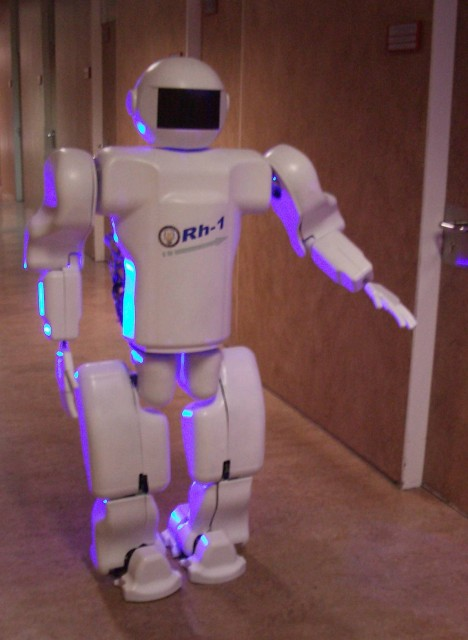
\includegraphics[scale=0.25]{rh1.jpg}
\caption{Rh-1 humanoid robot}
\label{fig:rh}
\end{figure}
